%!TEX root = /Users/louis/Documents/PhD/Deliverables/Thesis/thesis.tex

\section{Research Method}
\label{sec:research_method}
To explore the hypothesis outlined above, the thesis research was conducted using the method described in this section and summarised in Figure~\ref{fig:research_method}. The shaded boxes represent the three \emph{phases} of research, which are described below. The unshaded boxes represent inputs and outputs to those phases.

\begin{figure}[htbp]
  \begin{center}
    \leavevmode
    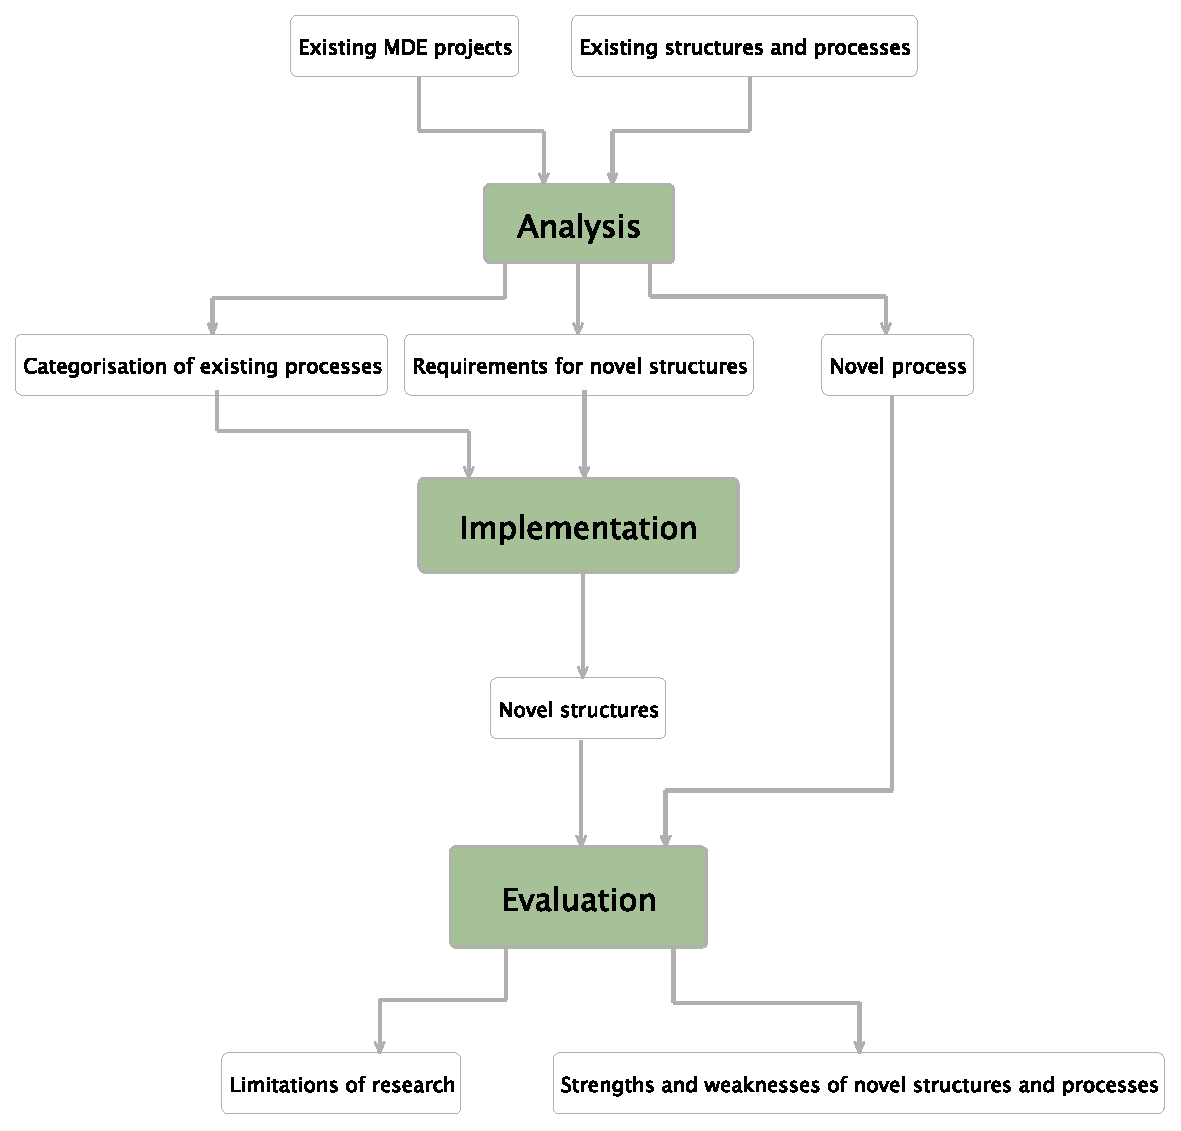
\includegraphics[width=12cm]{1.Introduction/images/method.pdf}
  \end{center}
  \caption{Overview of the research method.}
  \label{fig:research_method}
\end{figure}


Firstly, the \emph{analysis} phase involved studying the evolution of MDE development artefacts in existing projects. The results of the analysis phase were used to determine a category of evolution that lacked support in contemporary MDE development environments, \emph{model-metamodel co-evolution} or, simply \emph{co-evolution}. Co-evolution examples from existing MDE projects were used to categorise existing processes for managing co-evolution, and to formulate requirements for new structures and processes for managing co-evolution. The analysis phase also led to the identification of \emph{user-driven co-evolution}, a process for managing co-evolution that has not previously been recognised in the co-evolution literature.

The \emph{implementation} phase involved proposing, designing and implementing novel structures for managing co-evolution, and integrating the structures with a contemporary MDE environment. The co-evolution examples identified in the analysis phase were used for testing the implementation of the structures.

The \emph{evaluation} phase involved assessing the novel structures for managing co-evolution by comparison to existing structures, and demonstrating the novel process. Evaluation was performed using further examples of co-evolution. To mitigate a possible threat to the validity of the research, the examples used in the evaluation phase were different to those used in the analysis phase. The strengths and weaknesses of the novel and existing structures and processes were synthesised from the comparisons, particularly with respect to the productivity of the development activities that are used to manage co-evolution.

A similar method was used successfully in \cite{dig07thesis} to explore the extent to which component-based applications can be automatically evolved. Initially, \cite{dig06apis} conducted \emph{analysis} to identify and categorise evolution in five existing component-based applications, with the hypothesis that many of the changes could be classified as behaviour-preserving. By using examples from the survey, \cite{dig06detection} were able to \emph{implement} an algorithm for automatically detecting behaviour-preserving changes. The algorithm was then used to implement tools for migrating code in a distributed and collaborative software development environment \cite{dig06automatic}, and for analysing the history of component-based applications \cite{dig07cms}. The latter facilitated better understanding of program evolution, and refinement of the detection algorithm. Finally, \cite{dig07thesis} \emph{evaluated} the tools and detection algorithm by application to three further component-based applications.